\chapter{Implementation}
\label{sec:implementation}
This section discusses key concepts of the approximate distance oracles
implementation made to perform the experiments, and highlights obstacles
and solutions found while developing the implementation. Throughout
the implementation phase, I have tested my solution and benchmarked
my improvements against a graph based on friend lists from Facebook.
The graph has 4039 vertices, 88243 edges, and can be found here
\url{http://snap.stanford.edu/data/egonets-Facebook.html}. This graph I refer
to as the Facebook or test data set.\\\\
All the code is available at \url{https://github.com/brunsgaard/ado}.

\section{Choice of programming language}
The initial attempt to implement approximate distance oracles was done in
Python, but due to extreme memory consumption I reimplemented the algorithm
in C++. \autoref{tab:py_vs_cpp_fb} compares the final C++ implementation of
\proc{prepro} against vanilla Python. C++, as a compiled and heavily optimized
language, has an inherent performance advantage over Python which is an
interpreted language.

Using Google SparseHash\footnote{The Google SparseHash project contains
several hash-map implementations in use at Google, with different performance
characteristics, including an implementation that optimizes for space and
one that optimizes for speed. \url{https://code.google.com/p/sparsehash/}
} 
and multi-threaded processing, the C++ implementation greatly improves both memory
pressure and run times compared against Python.

\begin{table}[htbp]
    \centering
    \begin{tabular}{ l | c | c }
        \toprule
        lang & space & runtime\\
        \midrule
        Python & 118Mb & 39s\\
        C++ & 13Mb & 1s\\
        \bottomrule
    \end{tabular}
    \caption{Performance comparison between C++ and Python implementation,
             when run on \proc{prepro} on facebook test data.}
    \label{tab:py_vs_cpp_fb}
\end{table}

Due to the size of the graphs I use in the experiment, I need low memory
overhead and control over allocation. The memory pressure rapidly increases
with the number of nodes/edges, to the point where a graph with 30000 vertices
and 150000 edges, was barely able to compute with Python on a modern Macbook
pro. The data for which I have to run my experiments is much larger, and thus
the Python implementation was discarded.

\section{Data structures}

The graph is represented as an adjacency list, using a STL\footnote{Standard
Template Library container classes etc for C++, see more at
\url{http://www.sgi.com/tech/stl/stl_introduction.html}} \texttt{vector}
representing the vertices, and a STL \texttt{forward list} (one-way linked
list) for edges. An edge is a \texttt{struct} with just two members, a
memory managed pointer to the vertex and a weight, represented as a double.
\autoref{fig:graph-code-head} show the types and type definition used in the
final solution.

\begin{figure}
\lstset{language=C++}
\begin{lstlisting}
typedef double Weight;
const Weight MaxWeight = std::numeric_limits<double>::infinity();
typedef std::vector<std::shared_ptr<Vertex>> VertexVector;
typedef VertexVector::size_type VertexId;

struct AdjacentNode
{
  std::shared_ptr<Vertex> vertex;
  Weight weight;
  AdjacentNode(std::shared_ptr<Vertex> v, Weight w) : vertex(v), weight(w) {

  }
};

struct Vertex
{
  std::forward_list<AdjacentNode> adjacent;
  VertexId id;
  Vertex(VertexId i) : adjacent(), id(i) {
  }
};
\end{lstlisting}
\caption{graph.h: Code header defining the graph types}
\label{fig:graph-code-head}

\end{figure}

Because all data sets use positive integers as vertex ids, I can use a
\texttt{vector} to represent it, enabling fast constant time lookups. 
However the vector must be initialized in a special way.

First the input data is sequentially scanned to find the largest vertex
id. Then the vector is initialized with nodes from $0$ to the largest
vertex id. I perform an extra vertex allocation for the vertex added, and used
as source when finding the shortest path between $i$-centers and vertices as
mentioned in \autoref{sec:ado:creation}. By allocating it under initialization I
can avoid resizing the vector.

The precision of the \texttt{Weight} is reduced from a double to a float, and
the Vertex ids are reduced from a 64 bit to a 32 bit unsigned integer, when
storing the approximate distance oracle, thus cutting their memory consumption
in half.

\subsection{Preprocessed data}

For the actual data structure I need very memory efficient hash maps, since I 
will be storing a hash map (the cluster) for each node in the graph. Most of
these hash maps will be very sparse, however a few ($w \in A_{k-1}$) will be
dense.

I use Google SparseHash for these hash maps, since it uses an underlying
bitmap improving efficiency with empty buckets. What I gain in memory
efficiency I loose in runtime, so the implementation uses STL
\texttt{unordered\_map} until the very end of preprocessing where it will be
converted to Google's \texttt{sparse\_hash\_map}. \autoref{fig:memcompare}
show the memory consumption on the facebook dataset before and after applying
Google sparse hash to the implementation.

\begin{figure}
    \centering
    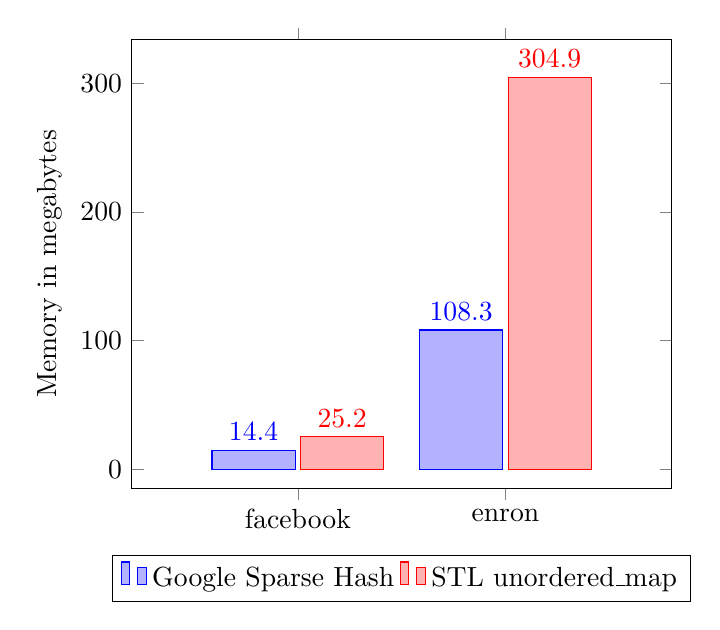
\begin{tikzpicture}
        \begin{axis}[
                ybar,
                legend style={at={(0.5,-0.15)},
                    anchor=north,legend columns=-1},
                ylabel=Memory in megabytes,
                symbolic x coords={facebook,enron},
                xtick=data,
                enlarge x limits={abs=60pt},
                bar width=30pt,
                nodes near coords,
                nodes near coords align={vertical},
                ]
            \addplot coordinates {(facebook,14.4) (enron,108.3) };
            \addplot coordinates {(facebook,25.2) (enron,304.9) };
            \legend{Google Sparse Hash,STL unordered\_map}
        \end{axis}
    \end{tikzpicture}
    \caption{Comparison of memory consumption using Google sparse hash and STL
        unordered respectively.}
    \label{fig:memcompare}
\end{figure}

When constructing the data structure, the output data from the modified
Dijkstra is the clusters, so the final step is the creation of bunches,
corresponding to line 11-12 in \autoref{pseudo:prepro}.

This requires the program to keep both clusters and bunches in memory,
effectively doubling the memory usage during the last step. There is no
need for me to convert the clusters into bunches, as I can just access the
information I need in the clusters directly, because I have global access to
all clusters.
This is also mentioned in \autoref{sec:ado:creation}, where I explained that
bunches allows for distance labeling. In my case I have a global state and
can access all information from the clusters directly, thus I do not need
to create bunches. To use the clusters directly, I make a small modification
to the \proc{dist} algorithm in \autoref{pseudo:dist}. The modification is
shown in \autoref{pseudo:dist_mod}, only line 3 has changed.

\begin{figure}[htbp]
\begin{codebox}
    \Procname{$\proc{dist\_mod}_{k}(u, v)$}
    \li $w \gets u$
    \li $i \gets 0$ 
    \li \While $v \notin C(w)$
    \li     \Do
                $i \gets i+1$
    \li         $(u,v) \gets (v,u)$
    \li         $w \gets p_{i}(u)$
            \End
    \li \Return $\delta(w,u) + \delta(w,v)$
\end{codebox}
\caption{The modified distance query algorithm}
\label{pseudo:dist_mod}
\end{figure}

By outputting the clusters to a file I avoid both preprocessing them every
time and keeping them in memory, during processing. Thus the only memory I
need is for a single cluster (or the number of threads calculating clusters),
and a bit for the graph and witnesses. The biggest data set with 1965206
nodes and 2766607 edges uses 1.4 GB memory during cluster creation with
8 threads, well with-in the expectations of modern computers. Before the
clusters were discarded after being written to the output file, memory usage
was in excess of 50 GB, but the program still terminated given enough swap
space (if the bunch creation was left out, otherwise the operating system
killed the process).

For the output files, a custom file format was created for the witnesses and
clusters. To avoid spending cpu cycles on formatting, the data is simply
\emph{reinterpret\_cast}'d to \texttt{unsigned chars}, which means the program
simply treats the memory of an e.g. 4 byte 32-bit integer as 4 bytes of
characters, which can be written directly to a file. For the witnesses this
means that every witness it outputted as a fixed size struct, each containing
the following: $i$-center reference, vertex id, distance and vertex reference
\autoref{tab:witness_ff}. There is no header or delimiter and the number of
bytes used to represent a witness is determined by the underlying types, so if
a type is changed, data structures previously created will be unreadable and
must be re-created.

\begin{table}[htbp]
    \centering
    \begin{tabular}{ | c | c | c | c |}
        \hline
        icenter reference & vertex id & distance & vertex reference.\\
        \hline
        4 bytes (int) & 8 bytes (uint64) & 8 bytes (double) & 8 bytes (int64)\\
        \hline
    \end{tabular}
    \caption{file format of witness, bytes counts are dynamic and/or compiler
             implementation specific}
    \label{tab:witness_ff}
\end{table}

For the clusters I used the built-in Google
SparseHash serializer\footnote{\url{
http://sparsehash.googlecode.com/svn/trunk/doc/sparse\_hash\_map.html\#io}}, 
but combined all clusters into a single file, by adding a header before the
serialized data. This header is 8 bytes (the size of two \texttt{uint32}), and
contains the source vertex id and a 32 bit unsigned integer which represents
the size of the serialized data, after Google SparseHash has serialized it
\autoref{tab:cluster_ff}. Google SparseHash's internal serializing format
includes a built-in delimiter, so multiple hash maps can be stored in same
file, but I still need the custom made size header, because I am reading the
same file from multiple threads \autoref{sec:file_read}.

\begin{table}[htbp]
    \centering
    \begin{tabular}{ | c | c | c |}
        \hline
        vertex id & size n & Google sparse hash \\
        \hline
        4 bytes (uint32) & 4 bytes (uint32) & n bytes (transparent data)\\
        \hline
    \end{tabular}
    \caption{File format of clusters}
    \label{tab:cluster_ff}
\end{table}

\section{Program execution optimization}

In order to optimize execution times, without having to worry too much about
multi-threaded programming, the implementation uses Intel® Threading Building
Blocks (TBB) and C++11 thread features. The only downside to using TBB is the
program is going to be optimized for Intel® CPUs, but recent updates to TBB
includes support for other x86/x86\_64 too.

\subsection{Concurrent preprocessing}\label{sec:multithread_compute}

Since all STL containers are thread safe when one does not mutate them, I can
easily use concurrency to utilize multiple CPU cores while preprocessing the
data. TBB's \texttt{parallel\_for} loop, automatically divides the for loop
work into smaller chunks and spawns the optimal amount of threads, which it
manages. This feature has been used to compute the clusters in parallel.

For writing the data structure to the output file, I need to add thread
safety. This is easily handled by simple mutex lock. Experiments show that
this mutex does not cause lock contention since I am not bottlenecked by
the file output and serialization blocks in the code. If I where, the
serialization could be moved outside the mutex, by serializing to a buffer
first, rather than directly to the file.

\subsection{Concurrent file reading and deserializion}\label{sec:file_read}

The reading and deserialization of Google SparseHash hashmaps is also done
concurrently. For this I use a TBB's \texttt{concurrent\_hash\_map} as the
data structure, because the STL containers are not thread safe for any
non-const methods (mutating).

Each thread \texttt{fopen(3)} the input file in read mode, and reads the
element header. It examines the hash map to check if the vertex id has
already been processed, and if so, skips ahead in the file, corresponding
to the end of the serialized data, which it got from the size header
(\autoref{tab:cluster_ff}). Then it tries to insert the vertex id into
the \texttt{concurrent\_hash\_map}, if it fails then a race condition
occurred and it skips ahead like before. With this style of loading from
the same file, race conditions are very likely to occur, but this is a
non-issue due to the design of \texttt{concurrent\_hash\_map}, this is why
- for my usecase - \texttt{concurrent\_hash\_map} is better than TBB's
\texttt{concurrent\_unordered\_map}, which does not have the same kind of
insert operation.
